\documentclass[12pt]{article}

% imports %
\usepackage[ngerman]{babel} \usepackage[utf8]{inputenc}
\usepackage{amssymb} 
\usepackage{amsmath}
\usepackage[pdftex]{graphicx}
\usepackage{float}
\usepackage{floatflt}
\usepackage{url} %for urls 
\usepackage{fancyhdr} %for header and footer
\usepackage{geometry}
\usepackage{enumitem} %for enum label refs
\geometry{a4paper, top=25mm, left=30mm, right=25mm, bottom=40mm, headsep=10mm,
footskip=12mm}

% title %
\title{Bachelorarbeit Informatik\\ 3D-Visualisierung von Zeitreihen im
Energiekontext}
\author{Stefan Bechert}

% heading style %
\pagestyle{fancy}
\fancyhf{}
\lhead{\leftmark}
\rhead{\thepage}



\begin{document}

% title page
\thispagestyle{empty}
\begin{center}
	\begin{bfseries}
		Universität Leipzig\\
		Fakultät für Mathematik und Informatik\\
		Institut für Informatik
	\end{bfseries}
\end{center}
\vspace{4cm}
\begin{center}
 	\large{\textbf{3D-Visualisierung von Zeitreihen im Energiekontext}}
\end{center}
\vspace{3cm}
\begin{center}
	\LARGE{\textbf{Bachelorarbeit}}
\end{center}
\vspace{5cm}
\begin{tabular}{lp{18em}r}
	Leipzig, TODO, 2016 && vorgelegt von \\[0.4cm]
	&& Bechert, Stefan\\
	&& Studiengang Informatik \\
	&& Bachelor of Science
\end{tabular}

\vspace{2cm}
\begin{flushleft}
	\textbf{Betreuender Hochschullehrer: \\Dr. Stefan Kühne\\Fakultät für
	Mathematik und Informatik\\Institut für Informatik}
\end{flushleft}

\newpage
\thispagestyle{empty}
\tableofcontents \newpage

\section{Einleitung}
\thispagestyle{empty}
	\subsection{Motivation}
Zeitreihen sind für alle heutigen wissenschaftlichen Disziplinen von großer
Relevanz. Sei es zur Auswertung von Smart Meter Daten im Energiebereich oder der
Analyse und Vorhersage von Aktienkursen an der Börse, Zeitreihen eignen sich
immer dann wenn eine zeitliche Entwicklung empirisch betrachtet wird.
[vgl. 1, S. X]\\[0.4cm]
		
			\begin{floatingfigure}[r]{4cm}
					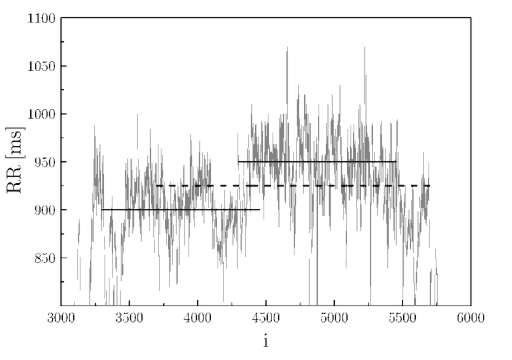
\includegraphics[width=2cm]{img/zeitreihe_2D_linie.jpg}
					\caption[2D]{Zweidimensionale
					Zeitreihendarstellung\footnotemark[1]}
			\end{floatingfigure}
		
			\footnotetext[1]{\url{http://www.max-schaldach-stiftung.de/.include/images/Stationaer.jpg},
			07.03.2016 }
	
		Im Rahmen der Auswertung von Zeitreihen sind verschiedene Darstellungsformen
		möglich, die jeweils ihre eigenen Vorteile mit sich bringen. Denkbar sind
		zweidimensionale oder dreidimensionale Darstellungen. In Ersterer ist ein
		Kennwert immer genau durch einen Zeitpunkt indentifizierbar.\\[0.4cm]
			
			
		Bei der dreidimensionelle Darstellung hingegen, kann man die Zeitreihe in
		Abhängigkeit von zwei zeitlichen Dimensionen auswerten.
		In Abbildung zwei zum Beispiel wird ein Kennwert nur jeweils durch ein Tupel
		aus Zins und Spalte eindeutig indentifiziert.\\[0.4cm]
		
			\begin{floatingfigure}[H]{4cm}
					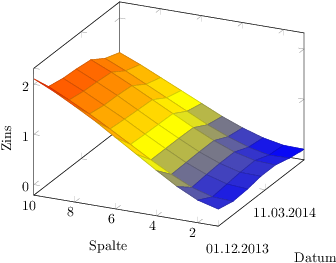
\includegraphics[width=2cm]{img/zeitreihe_3D.png}
					\caption[3D]{Dreidimensionale
					Zeitreihendarstellung\footnotemark}
			\end{floatingfigure}
			\footnotetext{\url{http://texwelt.de/wissen/upfiles/test_75.png},
					07.03.2016 }
		
		Ein Vorteil den diese Darstellung mit sich bringt, ist die Möglichkeit
		einzelne Spalten gegneinander zu vergleichen. So sieht man exemplarisch in
		Abbildung zwei, dass der Zins Anfang des Jahres 2014 in Spalte 10 bedeutend
		höher ist als Ende des Jahres.\\
		

		
		Ein weiterer Vorteil, der in Industrie und Wissenschaft große Bedeutung
		hat, ist, dass Ausschläge in den Daten in vielen Fällen sofort ins
		Auge fallen. Darunter könnten sich potentiell auch Fehler in den Daten
		befinden.\\[0.4cm]
		
		\hspace{0pt}
		\begin{floatingfigure}[l]{5cm}
					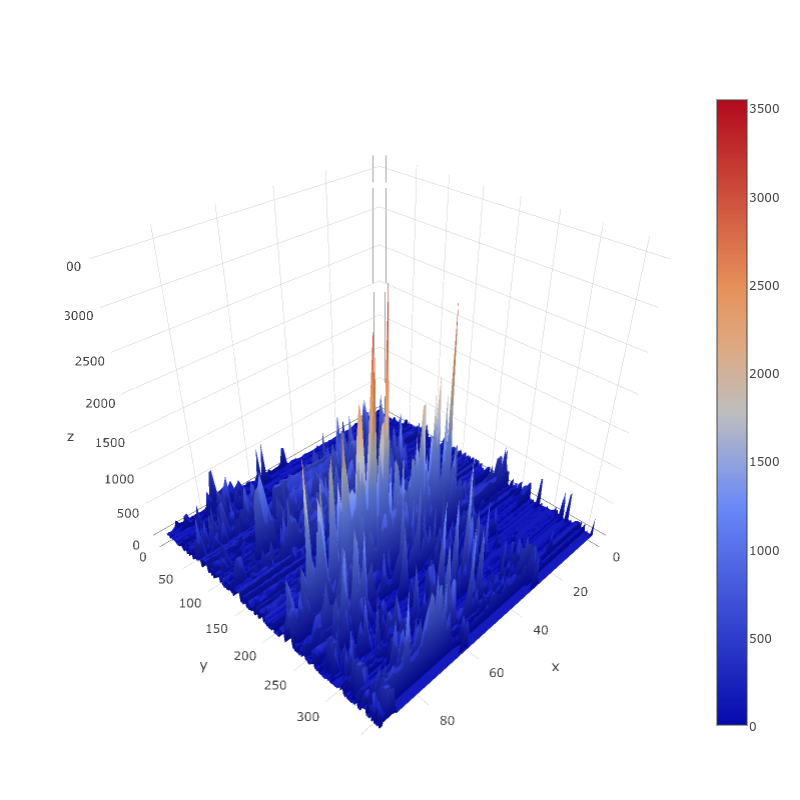
\includegraphics[scale=0.1]{img/zeitreihe_3D_fehler.png}
					\caption[3D-fehler]{Dreidimensionale
					Zeitreihendarstellung mit Ausschlägen}
			\end{floatingfigure}
		
		In Abbildung drei ist eine Zeitreihe zu sehen, bei der die
		Extrema in der Mitte der Daten deutlich sichtbar sind. Vergleiche
		hinsichtlich dem Unterschied zweidimensionale und dreimdimensionale
		Darstellung werden in Abschnitt 2.1 angeführt.\\
		
		
		\newpage
		
	\subsection{Zielsetzung}
		Ziel dieser Arbeit ist es vorhandene Webframeworks, die für die Darstellung
		von Zeitreihen entwickelt wurden und open source zugänglich sind, zu
		evaluieren und auf Basis eines davon eine Webkomponente zu bauen, die eine
		einfachere Auswertung von äquidistanten Zeitreihendaten ermöglicht.
		\paragraph{Analysis:}
		Bereits existierende Frameworks für Zeitreihendarstellung sollen hinsichtlich 
		den geforderten Zielen dieser Bachelorarbeit auf ihren Funktionsumfang 
		geprüft werden. Anhand dessen soll aufgezeigt werden welches Framework sich
		am ehesten für diese Arbeit eignet und welche Schritte dann in der
		Implementierung noch von nöten sind um die gewünschten Funktionalitäten
		umzusetzen.
		\paragraph{Functionality:}
		Die Komponente soll dem Benutzer ein Interface bereitstellen mit der
		die zeitlichen Dimensionen beliebig angepasst werden können. Um das zu realisieren 
		müssen vordefinierte Aggregatsfunktionen bereitgestellt werden. Desweiteren
		soll durch eine anpassbare Farbskala auch die Auswertung der Daten in der
		dritten Dimension, der Höhe, vereinfacht werden.
		\paragraph{Reusability:}
		Die Webkomponente soll ein in sich abgeschlossenes Modul werden, dass sich
		in verschiedenen Webapplikationen integrieren lässt. Aus diesem
		Grund soll die Software auf Basis von AngularJS
		\footnote{\url{https://angularjs.org/}} entwickelt und schließlich mit bekannten 
		Web-Build-Tools wie bower \footnote{\url{http://bower.io/}} oder npm
		\footnote{\url{https://www.npmjs.com/}} ausgeliefert werden.
		
	\newpage	
		
	\subsection{Gliederung}
		Die Arbeit ist in sechs Bestandteile gegliedert. Zu Beginn steht die
		Einleitung in der die Motivation für diese Arbeit erläutert und die Ziele, die erfüllt
		werden sollen, gesetzt werden.\\[0.4cm]
		Darauf folgt der Analyse-Abschnitt. Relevante Anwendungsszenarien
		werden simuliert und ausgewertet. Ziel ist es sowohl nochmals den Mehrwert,
		den diese Arbeit bietet, genauer herauszuarbeiten als auch Ziele der
		entstehenden Software zu spezifizieren. Desweiteren werden Frameworks, die als Grundlage
		dienen können, analysiert und zum Schluss eine Machbarkeitsstudie
		durchgeführt.\\[0.4cm]
		Den dritten Teil dieser Arbeit bildet ein Grundlagenkapitel. Hier werden
		wichtige Begrifflichkeiten definiert und die logischen Überlegungen, auf denen
		die Software aufgebaut seien wird, erläutert.\\[0.4cm]
		Im folgenden Kapitel, dem Konzept, werden Vorüberlegungen getroffen nach
		welchem Muster entwickelt werden soll. Wird ein Vorprojekt entwickelt? Wird
		test-first Development eingesetzt? Welche Programmierparadigmen werden zu
		Grunde gelegt? Diese Fragen werden beantwortet.\\[0.4cm]
		Danach folgt die Dokumentation des eigentlichen Implementierungsprozesses.
		Wichtige Fragen und Entscheidungen in der technischen Umsetzung werden hier
		diskutiert.\\[0.4cm]
		Zu guter Letzt folgt eine Auswertung der Arbeit. Es wird evaluiert ob die
		geforderten Ziele erreicht wurden und welche weiteren Ideen auf Basis der hier
		entwickelten Software perspektivisch umgesetzt werden könnten.
		
	\newpage	
		
\section{Analyse}
	In der Analyse werden Anwedungsszenarien vorgestellt anhand deren die genauen
	Anforderungen an die Software formuliert werden. Desweiteren werden
	Webframeworks auf die ermittelten Anforderungen hin untersucht und auf Basis
	dessen, eines davon als Grundlage für die Implementierung ausgewählt. Zum
	Schluss folgt eine Machbarkeitsstudie.

	\subsection{Anwendungsszenarien}
		\subsubsection{Smart Meter Strom Zeitreihe}
			Viele Energielieferanten nutzen schon seit über zwei Jahrzehnten sogenannte
			"`intelligente"' Zähler. Was früher hauptsächlich für Großunternehmen
			eingesetzt wurde findet heute auch immer mehr Gebrauch in
			Privathaushalten.\\[0.3cm]
			Während herkömmliche Stromzähler lediglich die Summe des verbrauchtes Stroms
			messen, ermöglichen es "`intelligente"' Zähler, englisch Smart Meter
			genannt, auch Informationen darüber zu geben, wann wie viel Strom verbraucht
			wurde. Durch die Einbindung der Smart Meter in Kommunikationsnetze wird
			außerdem häufiges Auslesen der Daten für den Energeilieferanten
			kostengünstiger. Auf diese Weise entstehen Zeitreihen, die den Verbrauch
			an einem Anschlusses mit einem gegeben Takt in einem bestimmten Zeitraum
			widerspiegeln.\\[0.3cm]
			Auf Basis dieser Daten kann der Energielieferant für sich wichtige
			Auswertungen vornehmen. Tarife können verbrauchsspezifisch auf den Endkunden
			angepasst werden.
			\footnote{vgl.\url{https://www.bmwi.de/BMWi/Redaktion/PDF/Publikationen/Studien/kosten-nutzen-analyse-fuer-flaechendeckenden-einsatz-intelligenterzaehler,property=pdf,bereich=bmwi2012,sprache=de,rwb=true.pdf}}
			Oder durch die gewonnenen Daten können Verbesserung am Stromnetz, wie
			zum Beispiel die Optimierung von Stromspeichern, durchgeführt
			werden.\\[0.3cm]
			Im Folgenden soll ein Szenario betrachtet werden, bei dem eine Smart Meter
			Zeitreihe eines Endkunden in 1-Stunden Intervallen über ein Jahr gegeben
			sei. Mögliche Fragen, die ein Analyst bei der Auswertung dieser Daten für
			sein Energieunternehmen stellen könnte, wären:
			
			\begin{enumerate}
			  \item Wie viel Strom wurde im gesamten Jahr verbraucht?
			  \item In welchem Monat wurde durchschnittlich am meisten/wenigsten Strom
			  verbraucht?
			  \item Haben die Daten Fehler?
			  \item Gibt es ein starkes Verbrauchsgefälle zwischen Arbeitstagen und
			  Wochenenden?
			  \item Bleibt der Verbrauch über einen Monat hin nahezu konstant?
			  \item Wie sieht der Verbrauch in der ersten Woche genau aus?
			\end{enumerate}
			
			
			\begin{figure}[hb]
					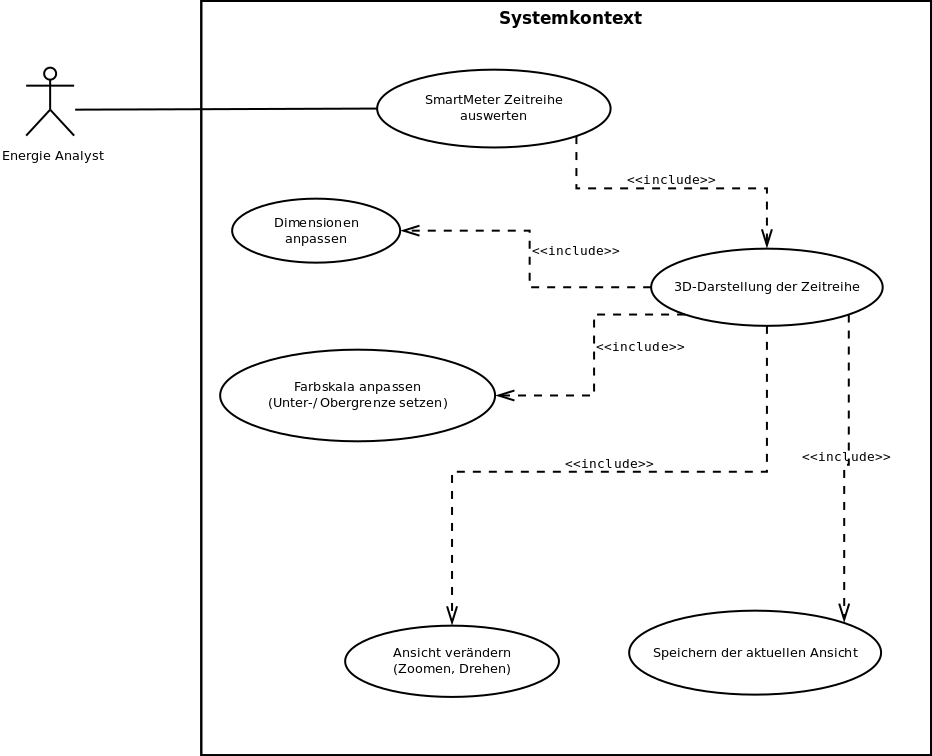
\includegraphics[width=1.0\textwidth]{dia/usecase-smartmeter.png}
					\caption[smartmeter]{Anwendungsfall SmartMeter}
			\end{figure}
			
		\subsubsection{Emissionsfaktoren der Stromerzeugung - 14 Jahre}
		
			\url{http://www.iinas.org/tl_files/iinas/downloads/GEMIS/2007_Emi-Daten_AGEEStat-ZSW.pdf}
	\subsection{Anforderungsanalyse}
		Auf Basis der vorgestellten Szenarien werden hier funktionale-, wie auch
		nicht-funktionale Anforderungen festgehalten.
		\subsubsection{Funktionale Anforderungen}
			Funktionale Anforderungen beschreiben in der Sprache des Systems die
			Funktionen, die ein System bereitstellen soll [vgl. 2, S. 29]. Im Folgenden
			werden use cases erstellt, die die Abläufe aus den oben genannten Szenarien
			verallgemeinern sollen. Das System (bzw. die Software) wird spezifischer als
			\textit{Komponente} betitelt. Die Durchnummerierung dient dem
			besseren Bezug in der Auswertung am Ende der Arbeit.
			\begin{enumerate}
			  \item{
			  	Dreidimensionale Darstellung einer Zeitreihe.\\[0.2cm]
			  	Die Komponente soll eine Zeitreihe in einem von ihr vordefinierten
			  	Format annehmen und dreidimensional darstellen können.}
			  \item{
			  	Bewegung im dreidimensionalen Raum.\\[0.2cm]
			  	Die Komponente soll dem Nutzer ermöglichen die Kamera in der Darstellung
			  	zu bewegen. Dazu zählt sowohl Rotation als auch Verschiebung auf allen
			  	drei Achsen.}
			  \item{
			  	Anpassung der Farbskala.\\[0.2cm]
			  	Die Komponente soll dem Nutzer ermöglichen die Farbskala aus einer großen
			  	Auswahl von Skalen auszuwählen. Desweiteren soll eine Möglichkeit bereit
			  	gestellt werden, die Unter- und Obergrenze beliebig zu setzen.}
			  \item{
			  	Verändern der Zeitachsen.\\[0.2cm]
			  	Beide Zeitachsen sollen vom Nutzer im Rahmen, den die gegebene Zeitreihe
			  	vorgibt, angepasst werden können. Für diese Anforderung wird \ref{agg}.
			  	benötigt.}
			  \item{\label{agg}
			  	Bereitstellen von Aggregationsfunktionen.\\[0.2cm]
			  	Die Komponente soll dem Nutzer Aggregationsfunktionen für Summe,
			  	Durschnitt, Maximum und Minimum zur Verfügung stellen.}
			\end{enumerate}
		\newpage	
		\subsubsection{Nicht-Funktionale Anforderungen}
			Nicht-Funktionale Anforderungen, oder auch Qualitätsanforderungen, legen die
			qualitativen Eigenschaften, die das System leisten soll, fest. Sie beziehen
			sich auf die oben genannten funktionalen Anforderungen und besitzen die
			Eigenschaft nur schwer spezifizierbar, bzw. testbar zu sein [vgl.
			2, S. 29 - 30]. Folgende nicht-funktionale
			Anforderungstypen werden unterschieden [vgl. 3, S. 249 - 250]:
			\begin{itemize}
			  \setlength{\itemsep}{2pt}
			  \item[--] Aussehen und Handhabung
			  \item[--] Benutzbarkeit
			  \item[--] Sicherheit
			  \item[--] Leistung
			  \item[--] Wartbarkeit
			  \item[--] Übertragbarkeit
			  \item[--] Politische oder Kulturelle Umgebungsbedingungen
			  \item[--] Gesetzliche Vorgaben
			\end{itemize}
			Für die Komponente sind allerdings nur die Folgenden von Wichtigkeit:
			
			\paragraph{Aussehen und Handhabung} $\;$ \\[0.3cm]
			Aussehen und Handhabung befassen sich nicht direkt mit den Details des
			Designs sondern legen viel mehr fest, welchen Eindruck die Komponente
			vermitteln soll [vgl. 3, S. 250].\\[0.2cm]
			Bei der zu entwickelnden Komponente wird der Hauptfokus im Bereich Aussehen
			und Handhabung auf ein schlichtes Design gesetzt, das es später ermöglicht,
			die Komponente in verschiedene Webanwendungen zu integrieren ohne deren
			Grunddesign zu stören. Desweiteren, da die Aufgabe dieser Komponente im
			Bereich der Visualisierung liegt, ist es ebenfalls wichtig, dem
			Interface, das die Komponente mit sich bringt, den Eindruck zu verleihen, die
			Komponente wäre nach dem aktuellen Stand der Technik (engl. state of the art
			[vgl. 3, S. 250]) designt worden.
			
			\paragraph{Benutzbarkeit} $\;$ \\[0.3cm]
			Benutzbarkeit ist eine der Schlüsseleigenschaften, die entscheiden, ob die
			Software später von Benutzern, für die sie entwickelt wurde, genutzt wird
			[vgl.
			3, S. 253]. Eine schlechte Benutzbarkeit kann trotz vollstäniger
			Funktionalität und gegebener Korrektheit zur Ablehnung der Software
			führen.\\[0.2cm]
			Da die zu entwickelnde Komponente Open Source ausgeliefert werden soll,
			um in verschiedenen Webapplikationen Anklang zu finden, ist es wichtig, die
			Benutzbarkeit der Komponente für verschiedene Endbenutzer sicherzustellen. 
			Interesse an dieser Software haben hauptsächlich Benutzer, welche Zeitreihen
			auf verschieden Aspekte hin auswerten wollen. Das fordert zwar inhaltliches 
			Wissen über die Auswertung, setzt allerdings nur die üblichen Kompetenzen im 
			Umgang mit Computern vorraus. Insofern soll die Komponente für gerade diese 
			Benutzer einfach zu lernen sein.
			
			\paragraph{Skalierbarkeit} $\;$ \\[0.3cm]
			Skalierbarkeit beschreibt, wie performant Software mit Änderungen in der
			Datengröße umgehen kann. Hinsichtlich der Tatsache, dass Zeitreihen
			beliebige Größenausmaße annehmen können, muss auch die Komponente mit solchen
			Änderungen umgehen können. Da die Komponente allerdings im
			Rahmen einer Webapplikation auf der Hardware des Endbenutzers laufen wird,
			lassen sich an dieser Stelle keine konkreten Angaben zu der Größe und der
			Zeit, in der die Operatioenn ablaufen, treffen. TODO (vlt Vergleichssystem
			wählen oder mit Komplexität festsetzen: doppelte Datengroesse = doppelte
			Zeit?)
			
			\paragraph{Übertragbarkeit} $\;$ \\[0.3cm]
			Wie oben erwähnt, soll die Komponente Open Source für andere
			Webapplikationen zur Verfügung stehen. Im Rahmen dessen muss die Komponente
			die geforderten Umgebungsbedingungen, der Webapplikationen erfüllen. Ziel ist
			es, die Komponente in jedem Browser, der WebGL unterstützt, verwenden zu
			können. Desweiteren soll die Übertragbarkeit verbessert werden, indem die
			Komponente für Webentwickler über öffentliche Paket Manager ausgeliefert
			wird.
			
			\paragraph{Korrektheit} $\;$ \\[0.3cm]
			Zu guter Letzt spielt die Korrektheit als nicht-funktionaler Anforderungstyp
			eine große Rolle für die Komponente. Die erfolgreiche und korrekte Auswertung
			einer Zeitreihe ist nur dann möglich, wenn die Daten richtig verarbeitet
			und visualisiert werden. Fehler in der Darstellung oder der Umrechnung würden
			zu falschen Schlussfolgerungen führen und könnten schwerwiegende Konsequenzen
			für den Endbenutzer mit sich bringen.
			
			\newpage
	\subsection{Webframeworks zur Zeitreihendarstellung}
		\subsubsection{dygraphs}
		\subsubsection{Plotly}
		\subsubsection{x3dom}

		\subsubsection{Fazit}
	\subsection{Machbarkeitsstudie}
\section{Entwurf}
		Welche theoretischen und praktischen Grundlagen sind zur Umsetzung dieser Arbeit erforderlich?
	\subsection{Zeitreihen, Repräsentationen und Operationen}
		\subsubsection{Definition Array}
		Sei $n \in \mathbb{N}$. Ein \textbf{Array} $arr = [a_{0}, a_{1}, ..., a_{n-1}]$ ist eine endliche Abfolge von Werten, die ueber ihren Index $i$ referenziert werden. Es gilt $arr[i] = a_{i}$, wobei $i \in \{0,1, ..., n-1\}$. \\[0.2cm]
		Die \textbf{Länge} eines Arrays $|arr|$ entspricht der Anzahl der Werte in $arr$, also $|arr| = n$.\\[0.4cm]
		Sei $arr$ ein Array. Falls ein $i \in \{0,1, ..., |arr| - 1\}$ existiert sodass $arr[i]$ selbst ein Array ist so heisst $arr$ \textbf{geschachtelt} und $arr[i]$ Unterarray von $arr$. Ansonsten heisst $arr$ \textbf{nicht geschachtelt}.\\[0.4cm]
		Sei $arr$ ein Array. Die Menge $\boldsymbol{\chi(arr)}$ ist die Menge aller Arrays in $arr$ und deren rekursiv erreichbaren Unterarrays, die selbst nicht geschachtelt sind. (Eigentlich muesste man das besser ausdruecken)
		\subsubsection{Definition Zeitreihe}
		\label{sec: def}
		Eine \textbf{äquidistante Zeitreihe} ist ein Tripel 
			\begin{equation}
				D^{2} = (V, i, s)
			\end{equation}
		wobei
			\begin{equation}
				V = [v_{0}, v_{1}, ..., v_{n - 1}]
			\end{equation}
		ein Array aus n Kennwerten darstellt.
		$i$ beschreibt den zeitlichen Abstand zwischen zwei Kennwerten in Millisekunden und s repräsentiert den Starzeitpunkt der Zeitreihe in 		Millisekunden seit dem 01.01.1970.
		\subsubsection{Repräsentationen}
			\paragraph{2D - Repräsentation}
				Die Repräsentation nach \ref{sec: def} ist eine 2-dimensionale Darstellung der Kennzahlen, da nur ein Index benoetigt wird um jede Kennzahl 						eindeutig zu referenzieren.
				
			\paragraph{3D - Repräsentation}
				Jede Zeitreihe kann auch in Abhängigkeit von zwei unterschiedlichen Zeitdimensionen angegeben werden. \\[0,3cm]
				Sei $D^{2} = (V, i, s)$ eine Zeitreihe in 2D-Repräsentation. So lässt sich diese Zeitreihe auch darstellen in 3D-Repräsentation als
				\begin{equation}
					D^{3} = (V', i, s)
				\end{equation}
				mit
				\begin{equation}
					V' = [[v_{0}, v_{1}, ..., v_{t_{1} - 1}]_{0},[v_{0}, v_{1}, ..., v_{t_{2} - 1}]_{1},...,[v_{0}, v_{1}, ..., v_{t_{m} - 1}]_{m}]
				\end{equation}
				wobei 
				\begin{equation}
					\sum_{k=1}^{m}t_{k} = |V|.
				\end{equation}
				Falls
				\begin{equation}
					t_{1}=t_{2}=...=t_{m}
				\end{equation}
				gilt, so nennt man $V'$ eine \textbf{homogene}, ansonsten eine \textbf{inhomegene} 3D-Repräsentation von D.
			\paragraph{Folgerung Homogen 3D}
				Sei $D^{3}$ als homogen gegeben. So folgt:
				\begin{equation}
					\sum_{k=1}^{m}t_{k} = t*m = |V|.
				\end{equation}
				
			\paragraph{nD - Repräsentation, Ueberlegung}
				Allgemein kann man jede Zeitreihe in $n$ vielen Dimensionen darstellen (da beliebig kleine Zeitschritte), allerdings erreicht man dadurch irgendwann keine neuen Informationen mehr sondern ausschliesslich Kennwertduplizierung.
		\subsubsection{Operationen - allgemein}
			Sei $K^{n}$ die Menge aller Zeitreihen in $n$D-Repraesentation.		
		
			\paragraph{Unterteilung}
				$\forall n \geq 2$ gilt:\\
				Sei $D^{n} = (V, i, s)$ eine Zeitreihe in nD-Repraesentation.\\[0.0cm]
				Eine Unterteilung $\delta = (f, g)$ ist ein Tupel, wobei f eine Abbildung 
				\begin{equation}
					f: K^{n} \rightarrow K^{n+1}.
				\end{equation}\\[0.3cm]
				darstellt mit
				\begin{equation}
					f(D^{n}) = f ((V,i,s)) = (g(V), i, s)
				\end{equation}
				und
				\begin{equation}
					g(V) = g.replace(arr \in \chi(V), g(arr)).
				\end{equation}
				Sei $D^{n} = (V, i, s)$ homogen und $\delta(D^{n}) = D^{n+1} = (V', i, s)$.
				Eine Unterteilung heisst \textbf{homogen} falls ein $n \in \mathbb{N}$ exisitiert, sodass
				\begin{equation}
					\forall arr \in \chi(V'): |arr| = n.
				\end{equation}
				
			\paragraph{Aggregation}
				$\forall n \geq 3$ gilt:\\
				Sei $D^{n} = (V, i, s)$ eine Zeitreihe in nD-Repraesentation.\\[0.3cm]
				Eine Aggregation $\phi$ ist eine Abbildung 
				\begin{equation}
					\phi: K^{n} \rightarrow K^{n-1}.
				\end{equation}
				
			\paragraph{Aggregationsregeln}
				Sei $D^{n} = (V, i, s)$ eine Zeitreihe in nD-Repraesentation.\\[0.3cm]
			
				\begin{enumerate}
					\item{Eine Zeitreihe ist genau dann aggregierbar, wenn $n \geq 3$.}
					\item{Sei $D^{n} = (V, i, s)$ homogen. Fuer 
						\begin{equation}
							\phi(D^{n}) = D^{n-1} = (V', i', s)
						\end{equation}
						gilt 
						\begin{equation}
							i' = |\chi(D^{n})|*i
						\end{equation}
						.
					}
					\item{Sei $D^{n} = (V, i, s)$ inhomogen. Fuer
						\begin{equation}
							\phi(D^{n}) = D^{n-1} = (V', i', s)
						\end{equation}
						gilt 
						\begin{equation}
							i' = [l_{0}, l_{1}, ..., l_{|\chi(V)| - 1}]
						\end{equation}
						wobei $i'[0] = l_{0} = |\chi(V)[0]|$.
					}
				\end{enumerate}
				
			\begin{picture}(100,200)
				\put(0,140) {\line(1,0){180}}			
			
				% erste Spalte - Unterteilung
				\put(30,0) {$D^{n}$}
				\put(40,25) {\vector(0,-1){10}}
				\put(30,30) {$D^{n-1}$}
				\put(40,55) {\vector(0,-1){10}}
				\put(35,60) {...}
				\put(40,85) {\vector(0,-1){10}}
				\put(30,90) {$D^{3}$}
				\put(40,115) {\vector(0,-1){10}}
				\put(30,120) {$D^{2}$}
				\put(0,150) {\textbf{Unterteilung}}
				
				% zweite Spalte - Aggregation
				\put(130,0) {$D^{n}$}
				\put(140,15) {\vector(0, 1){10}}
				\put(130,30) {$D^{n-1}$}
				\put(140,45) {\vector(0, 1){10}}
				\put(135,60) {...}
				\put(140,75) {\vector(0, 1){10}}
				\put(130,90) {$D^{3}$}
				\put(140,105) {\vector(0, 1){10}}
				\put(130,120) {$D^{2}$}
				\put(100,150) {\textbf{Aggregation}}
			\end{picture}	

\section{Implementierung}
		Die Definition in \ref{sec: def} gilt im folgenden als die initiale Repräsentation einer Zeitreihe in der Anwendung. (Passt hier eig nicht, sollte eher zu Implementierung)\\
		
		Tatsaechliche Umsetzung: Probleme, Entscheidungen, 
	
				\paragraph{Wichtige Forderungen TODO aber merken}
				Dass die Teilarrays in der 3D Repraesentation die gleich Groesse haben ist fuer den spaeteren Render-Prozess von hoher Wichtigkeit, da andernfalls Daten in der Darstellung verloren gehen. Nichts destotrotz kann eine Zeitreihe auch in ungleiche Teile zerteilt werden (z.B. Monate), die allerdings zur Darstellung auf jeden Fall aggregiert werden muessen um die Forderung einzuhalten.
\section{Zusammenfassung und Evaluation}
	\subsection{Auswertung}
		Wurden die Ziele erfuellt? Wenn ja zeigen. Wenn nein, wieso nicht?
		Zeitpunkt: Nach der Fertigstellung der software.
	\subsection{Ausblick}
		Was koennte man aufbauend auf dieser Arbeit noch machen?
	
\newpage
\thispagestyle{empty}
\section*{Literaturverzeichnis}
\addcontentsline{toc}{section}{Literaturverzeichnis}

\begin{itemize}
  \item[] [1] Schlittgen, Rainer / Streitberg, Bernd H. J.: Zeitreihenanalyse.
  9. unwesentlich veränderte. Münchnen: Oldenbourg Verlag, 2001.
  \item[] [2] Ebert, Christof: Systematisches Requirements Engineering :
  Anforderungen ermitteln, spezifizieren, analysieren und verwalten.
  dpunkt.verlag, 2011.
  \item[] [3] Robertson, Susanne / Robertson, James: Mastering the Requirements
  Process: Getting Requirements Right. 3. Auflage. Amsterdam: Addison-Wesley,
  2012.
\end{itemize}

\newpage
\thispagestyle{empty}
\hspace{15cm}
\section*{\centering{Erklärung}}
	\vspace{5cm}
	\begin{center}
		Ich versichere, dass ich die vorliegende Arbeit selbständig und nur unter
 Verwendung der angegebenen Quellen und Hilfsmittel angefertigt habe,
insbesondere sind wörtliche oder sinngemäße Zitate als solche gekennzeichnet.
Mir ist bekannt, dass Zuwiderhandlung auch nachträglich zur Aberkennung
des Abschlusses führen kann
	\end{center}
	\vspace{3cm}
	\begin{tabular}{lp{4em}lp{4em}l}
 		Ort && Datum && Unterschrift
	\end{tabular}

\end{document}
